%%%%%%%%%%%%%%%%%%%%%%%%%%%%%%%%%%%%%%%%%
% Stylish Title Page
% LaTeX Template
% Version 2.0 (22/7/17)
%
% This template was downloaded from:
% http://www.LaTeXTemplates.com
%
% Original author:
% Peter Wilson (herries.press@earthlink.net) with modifications by:
% Vel (vel@latextemplates.com)
%
% License:
% CC BY-NC-SA 3.0 (http://creativecommons.org/licenses/by-nc-sa/3.0/)
%
% This template can be used in one of two ways:
%
% 1) Content can be added at the end of this file just before the \end{document}
% to use this title page as the starting point for your document.
%
% 2) Alternatively, if you already have a document which you wish to add this
% title page to, copy everything between the \begin{document} and
% \end{document} and paste it where you would like the title page in your
% document. You will then need to insert the packages and document
% configurations into your document carefully making sure you are not loading
% the same package twice and that there are no clashes.
%
%%%%%%%%%%%%%%%%%%%%%%%%%%%%%%%%%%%%%%%%%

%----------------------------------------------------------------------------------------
%	PACKAGES AND OTHER DOCUMENT CONFIGURATIONS
%----------------------------------------------------------------------------------------

\documentclass[12pt]{article}
\usepackage[UKenglish]{babel}
\usepackage[margin=1in]{geometry}


\usepackage[utf8]{inputenc}
\usepackage[T1]{fontenc}
\usepackage{import}
\usepackage{lwworksheets}
\usepackage{graphicx}


\begin{document}

\frontpage{Analogue Synthesiser}

%\import{../../worksheet-components}{title-page.tex}

\section{Soldering}
\label{sec:soldering}
\begin{instructions}
	\instruction{
		Read through \textit{all} these instructions thoroughly.
	}
	\instruction{
		Check and identify all components. Attach these with masking
		tape to the sheet lablled "Parts List" (Section
		\ref{sec:partslist}).
	}
	\instruction{
		You are now going to solder the components to the board using
		the instructions below.  You will need to refer to Section
		\ref{sec:placement} to see where each component should go.
	}

% Resistors

	\instruction{
		Solder the fifteen \ohm{1M} resistors, R25 - R39.
	}
	\instruction{
		Solder the eight \ohm{10k} resistors, R1, R2, R11 - 13, R16, R17 and R21.
	}
	\instruction{
		Solder the five \ohm{100} resistors, R40 - R44.
	}
	\instruction{
		Solder the four \ohm{100k} resistors, R8, R9, R14 and R15.
	}
	\instruction{
		Solder the three \ohm{1k} resistors, R3, R7 and R24.
	}
	\instruction{
		Solder the two \ohm{220k} resistors, R10 and R23.
	}

% Diodes

	\instruction{
		Solder the six 1N4148 diodes, D1 - D6. Make sure to line up the
		stripe on the circuit board with the black stripe on the diode.
		Check with a team member \textbf{before} soldering the first
		one.
	}

% IC Sockets

	\instruction{
		Solder the three 14-pin IC sockets for U1 - U3. Make sure to
		line the notch in the IC socket with the notch shown on the PCB.
		The pins are close together, so be careful not to bridge any.
	}
	\instruction{
		Solder the two 8-pin IC sockets for U5 and U6. Make sure to
		line the notch in the IC socket with the notch shown on the PCB.
		Again, be careful not to bridge any pins
	}

% Small capacitors

	\instruction{
		Solder the four 10nF capacitors, C5, C6, C11 and C12.
	}
	\instruction{
		Solder the two 1µF capacitors, C2 and C7.
	}
	\instruction{
		Solder the two 1nF capacitors, C3 and C8.
	}
	\instruction{
		Solder the 220nF capacitor, C4.
	}

% Taller components

	\instruction{
		Solder the headphones socket, J4. Only add solder to the holes
		that have metal coming out - no need to try and solder the plastic pins!
	}
	\instruction{
		Insert the five LEDs, D7 - D11. \textbf{Do NOT} solder them yet, and be
		careful to insert them the right way round: The flat edge on the
		outside of the LED should match the flat edge shown on the PCB.
		See Section \ref{sec:components} for a diagram.
	}
	\instruction{
		Get a member of team to check the orientation of the
		LEDs, then solder them in place.
	}
	\instruction{
		Ask a member of team for the relevant jig. Attach the two 20-pin
		headers to the jig and insert the headers into the board, then
		solder them in place. Be careful not to bridge any pins.
	}
	\instruction{
		Insert the two 10µF capacitors, C9 and C13. Make sure the
		white stripe on the capacitor is on the same side as the white
		patch on the PCB. Check with a member of team before soldering them.
		See the picture in Section \ref{sec:components} for an explanation.
	}
	\instruction{
		Insert the 100µF capacitor, C1. Make sure the
		white stripe on the capacitor is on the same side as the white
		patch on the PCB. Check with a member of team before soldering them.
	}

% Pots

	\instruction{
		Before soldering the potentiometers, ask a team member to check
		your soldering so far.
	}
	\instruction{
		Place the \ohm{50k} potentiometer into the slot for R18. \textbf{Do NOT} solder
		it yet.
	}
	\instruction{
		Get a team member to check the potentiometer is inserted in the
		correct place. Solder in place only once approval is given.
	}
	\instruction{
		Solder the seven \ohm{10k} potentiometers, R4 - R6, R19, R20, R22 and R45.
	}
	\instruction{
		Ask a member of team to check your soldering.
	}
\end{instructions}

\pagebreak
\section{Assembly}
\begin{instructions}
	\instruction{
		Fit ten rubber feet to the locations indicated on the bottom of
		the PCB.
	}
	\instruction{
		With a team member, insert the Pi Pico and all the integrated
		circuits. See Section \ref{sec:otherpartslist} for a list of which
		IC goes where. Make sure to insert them in the correct orientation.
	}
	\instruction{
		Connect a USB power source to the Pi Pico, headphones to the jack socket,
		and test your synthesiser! The LEDs should turn on when power is provided.
		Turn all the dials to half-way and press a key - sound should come out!
	}
	\instruction{
		Once it all works (and not before!), fit the knobs to the potentiometers.
	}
\end{instructions}

\section{Component Info}
\label{sec:components}

\explainLed
\explainDiode
\explainElectrolytic

\section{Schematic}

\includegraphics[width=0.9\textwidth]{img/sch-1.png}


\includegraphics[width=0.9\textwidth]{img/sch-2.png}

%\section{Etch}
%\label{sec:etch}
%
\includegraphics[width=\textwidth]{img/macropad-rev1-B_Cu_Oversized.png}

\section{Placement}
\label{sec:placement}
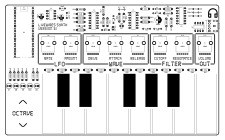
\includegraphics[width=0.8\textwidth]{img/component-layout.png}


%\section{Drill Sizes}
%\label{sec:drillsizes}
%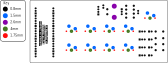
\includegraphics[width=\textheight,angle=90]{img/hole-colours.png}


\section{Solderable Parts List}
\label{sec:partslist}

\def\arraystretch{2}
\begin{tabular}{cccc}
\hline
\textbf{Reference}               & \textbf{Value}    & \textbf{Qty} & \textbf{Order Code} \\ \hline
C5, C6, C11, C12                 & 10nF              & 4            &                     \\ \hline
C2, C7                           & 1µF               & 2            &                     \\ \hline
C3, C8                           & 1nF               & 2            &                     \\ \hline
C9, C13                          & 10µF              & 2            &                     \\ \hline
C1                               & 100µF             & 1            &                     \\ \hline
C4                               & 220nF             & 1            &                     \\ \hline
R25 – R39                        & 1MΩ               & 15           &                     \\ \hline
R1, R2, R11 - R13, R16, R17, R21 & 10kΩ              & 8            &                     \\ \hline
R4 – R6, R19, R20, R22, R45      & 10kΩ              & 7            & PTV112-4420A-A103   \\ \hline
R40 – R44                        & 100Ω              & 5            &                     \\ \hline
R8, R9, R14, R15                 & 100kΩ             & 4            &                     \\ \hline
R3, R7, R24                      & 1kΩ               & 3            &                     \\ \hline
R10, R23                         & 220kΩ             & 2            &                     \\ \hline
R18                              & 50kΩ              & 1            & PTV112-4420A-B503   \\ \hline
D1 – D6                          & 1N4148            & 6            &                     \\ \hline
D7 – D11                         & Red               & 5            & 1573708             \\ \hline
J4                               & 3.5mm Jack        & 1            & 20-0137             \\ \hline
For U4                           & 20-pin socket     & 2            & 61302011821         \\ \hline
For U1 - U3                      & 14-pin DIP socket & 3            & 22-0108             \\ \hline
For U5 \& U6                     & 8-pin DIP socket  & 2            & 22-0107             \\ \hline
\end{tabular}




\section{Other Parts List}
\label{sec:otherpartslist}

\def\arraystretch{2}
\begin{tabular}{cccc}
\hline
\textbf{Reference}               & \textbf{Value}    & \textbf{Qty} & \textbf{Order Code} \\ \hline
U1 – U3                          & LM324N            & 3            & LM324N              \\ \hline
U4                               & Pi Pico           & 1            & SC0915              \\ \hline
U5                               & TC1044S           & 1            & TC1044SCPA          \\ \hline
U6                               & NJM4580D          & 1            & NJM4580D            \\ \hline
                                 & 20-pin header     & 2            & PH1-20-UA           \\ \hline
                                 & Rubber feet       & 10           & SJ5382-TRANSP       \\ \hline
                                 & MicroUSB cable    & 1            & 45-4009             \\ \hline
                                 & Headphones        & 1            & 220700              \\ \hline
                                 & Knobs             & 8            & -                   \\ \hline
                                 & Circuit board     & 1            & -                   \\ \hline
\end{tabular}


\end{document}
